\chapter{The DEF File: A Snapshot of Where Everything Lives}

\begin{tldr}
\begin{itemize}
  \item \textbf{Last chapter:} the tech file listed every legal shape on every layer. \textbf{This chapter:} the DEF records exactly which legal shapes ended up where, snapshot by snapshot through the flow.
  \item \textbf{DEF} (Design Exchange Format) is an ASCII file that captures the \textbf{current physical state} of the design: die shape, rows, instance placement, IO pin locations, and (later) full routing.
  \item DEF is emitted at \textbf{every major PD checkpoint} (post-floorplan, post-place, post-CTS, post-route); same file format, increasing completeness at each stage.
  \item \textbf{LEF + DEF together} give you enough to fully visualize a design in a layout viewer with no GDS in sight; GDS is for the fab, DEF is the working format used \emph{during} PD.
\end{itemize}
\end{tldr}

\begin{hook}
You have a netlist that says \emph{what} the design is and a LEF that says \emph{what each cell looks like}. Hand both to a tool and it still has no idea where to put anything. Somewhere there has to be a file that says \textbf{``this exact instance sits at (12.5, 7.5) microns, oriented north, and is fixed.''} That file gets rewritten after floorplan, after place, after CTS, after route. Same name. Same format. Different snapshot. What is inside it?
\end{hook}

\section{What DEF Actually Is}

\textbf{DEF} stands for \textbf{Design Exchange Format}. It is a plain-text file that describes the physical structure of a specific design instance: the die outline, the rows that standard cells slot into, the placement of every component, the IO pin locations on the boundary, and (after routing) the full wire and via geometry.

LEF tells the tool what a NAND2 cell physically looks like in the abstract. DEF tells the tool that instance \texttt{u\_alu/g\_carry} of that NAND2 sits at coordinate (12500, 7500) facing north. One is library, one is design.

\begin{keyidea}
A DEF file is a \textbf{textual snapshot of the design's physical state} at one point in the PD flow; LEF describes cells in the abstract, DEF describes \textbf{this design's instances} in concrete coordinates.
\end{keyidea}

\section{The Floorplan View}

The clearest mental picture of what DEF encodes is the floorplan itself. A die boundary, a core area inside it, IO pins around the edge, a few hard macros pre-placed, and standard cell rows filling the rest. Every one of those geometric facts has a DEF section behind it.

\begin{figure}[h]
\centering
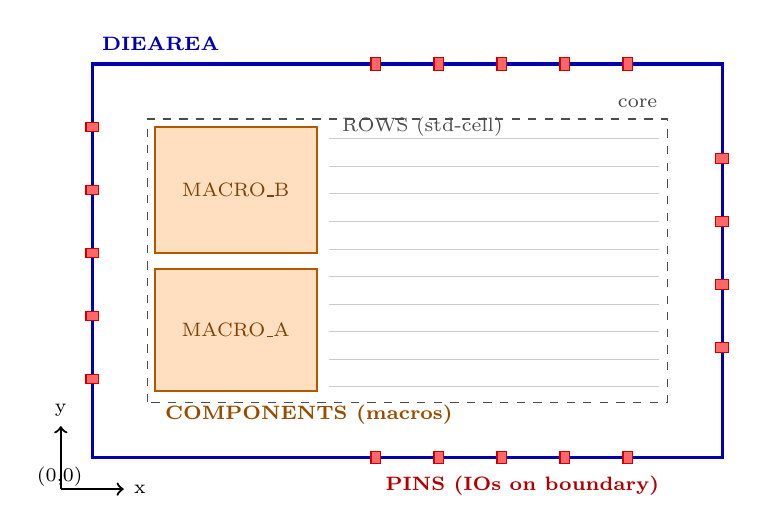
\begin{tikzpicture}[every node/.style={font=\scriptsize}]
  % DIEAREA
  \draw[very thick, blue!70!black] (0,0) rectangle (8,5);
  \node[blue!70!black, anchor=south west, font=\scriptsize\bfseries] at (0,5.05) {DIEAREA};

  % Core boundary
  \draw[dashed, gray!60!black] (0.7,0.7) rectangle (7.3,4.3);
  \node[gray!50!black, anchor=south east, font=\scriptsize] at (7.3,4.32) {core};

  % Standard cell rows
  \foreach \y in {0.9,1.25,1.6,1.95,2.3,2.65,3.0,3.35,3.7,4.05} {
    \draw[gray!40, line width=0.3pt] (3.0,\y) -- (7.2,\y);
  }
  \node[gray!60!black, anchor=west] at (3.05,4.2) {ROWS (std-cell)};

  % Macros
  \draw[fill=orange!25, draw=orange!70!black, thick] (0.8,0.85) rectangle (2.85,2.4);
  \node[orange!50!black] at (1.82,1.62) {MACRO\_A};
  \draw[fill=orange!25, draw=orange!70!black, thick] (0.8,2.6) rectangle (2.85,4.2);
  \node[orange!50!black] at (1.82,3.4) {MACRO\_B};
  \node[orange!60!black, anchor=west, font=\scriptsize\bfseries] at (0.8,0.55) {COMPONENTS (macros)};

  % IO pins around boundary
  \foreach \y in {1.0,1.8,2.6,3.4,4.2} {
    \draw[fill=red!60, draw=red!80!black] (-0.08,\y-0.06) rectangle (0.08,\y+0.06);
  }
  \foreach \y in {1.4,2.2,3.0,3.8} {
    \draw[fill=red!60, draw=red!80!black] (7.92,\y-0.06) rectangle (8.08,\y+0.06);
  }
  \foreach \x in {3.6,4.4,5.2,6.0,6.8} {
    \draw[fill=red!60, draw=red!80!black] (\x-0.06,-0.08) rectangle (\x+0.06,0.08);
    \draw[fill=red!60, draw=red!80!black] (\x-0.06,4.92) rectangle (\x+0.06,5.08);
  }
  \node[red!70!black, anchor=west, font=\scriptsize\bfseries] at (3.6,-0.35) {PINS (IOs on boundary)};

  % Origin marker
  \draw[->, thick] (-0.4,-0.4) -- (0.4,-0.4) node[right] {x};
  \draw[->, thick] (-0.4,-0.4) -- (-0.4,0.4) node[above] {y};
  \node[anchor=north east] at (0,0) {(0,0)};
\end{tikzpicture}
\caption{Floorplan-style picture of what a DEF file encodes. The die outline is the \textbf{DIEAREA} polygon, two pre-placed hard macros and the standard-cell rows live in \textbf{COMPONENTS} and \textbf{ROWS}, and the IO ports on the boundary are \textbf{PINS}. Each visible thing in this picture maps to one DEF section.}
\label{fig:def-floorplan}
\end{figure}

The DIEAREA polygon is walked \textbf{clockwise from the origin}, and order matters; reversing it flips the inside/outside semantics. The rows tile the inner core. The macros sit at fixed coordinates that the floorplanner has already committed to. The IO pads sit on the die edge.

\begin{hook}
Picture a \textbf{stage manager's set diagram} taped backstage: every prop (instance) has an X mark, every entrance (pin) is on the perimeter, every dancer's lane (row) is chalked across the floor. Lose the diagram mid-show and the next scene change collides two macros, which in silicon means DRC errors before you can spell ``re-floorplan.''
\end{hook}

\section{Inside the File}

Here is what the relevant sections look like in the actual ASCII. Names are illustrative; the keywords (\texttt{DIEAREA}, \texttt{ROW}, \texttt{COMPONENTS}, \texttt{PINS}, \texttt{NETS}) are not.

\begin{lstlisting}[style=eda,caption={Skeleton of a DEF file. Each major section ends with an explicit \texttt{END} keyword.},label={lst:def-skeleton}]
VERSION 5.8 ;
DIVIDERCHAR "/" ;
BUSBITCHARS "[]" ;
DESIGN top_block ;
UNITS DISTANCE MICRONS 1000 ;

DIEAREA ( 0 0 ) ( 0 38000 ) ( 14000 38000 )
        ( 14000 22000 ) ( 18000 22000 ) ( 18000 0 ) ;

ROW ROW_0 CORE 100 100 N DO 420 BY 1 STEP 200 1400 ;

COMPONENTS 4 ;
  - ENDCAP_L_0  TAPCELL_X1   + FIXED ( 100   100 ) N ;
  - u_alu/g_carry  NAND2_X1  + PLACED ( 12500 7500 ) N ;
  - u_alu/g_sum    XOR2_X2   + PLACED ( 13200 7500 ) FN ;
  - u_ctrl/fsm_q   DFFR_X1   + PLACED ( 4800  9100 ) S ;
END COMPONENTS

PINS 3 ;
  - clk + NET clk + DIRECTION INPUT + USE SIGNAL
        + LAYER M4 ( -70 0 ) ( 70 140 )
        + FIXED ( 9000 38000 ) N ;
  - rst_n + NET rst_n + DIRECTION INPUT + USE SIGNAL
        + LAYER M4 ( -70 0 ) ( 70 140 )
        + FIXED ( 11000 38000 ) N ;
  - q_out + NET q_out + DIRECTION OUTPUT + USE SIGNAL
        + LAYER M4 ( -70 0 ) ( 70 140 )
        + FIXED ( 18000 12000 ) E ;
END PINS

NETS 2 ;
  - n_carry ( u_alu/g_carry Z ) ( u_alu/g_sum A ) ;
  - clk     ( PIN clk ) ( u_ctrl/fsm_q CK ) ;
END NETS

END DESIGN
\end{lstlisting}

Note three things. First, every component line carries its \textbf{reference cell name} (so the tool can look the geometry up in LEF), its \textbf{placement status} (\texttt{FIXED} vs.\ \texttt{PLACED} vs.\ \texttt{UNPLACED}), and its \textbf{orientation} (\texttt{N}, \texttt{S}, \texttt{FN}, etc.). Second, the file lists a count after each section header (\texttt{COMPONENTS 4 ;}) so the parser can pre-allocate. Third, all coordinates are integers in DEF database units, not microns.

\begin{gut}
In Listing \ref{lst:def-skeleton}, which two instances are \textbf{fixed} and cannot be moved by the placer, and which can?
\gutans{\texttt{ENDCAP\_L\_0} is \texttt{FIXED} (physical-only end-cap cell, locked at floorplan time). The three logical instances (\texttt{u\_alu/g\_carry}, \texttt{u\_alu/g\_sum}, \texttt{u\_ctrl/fsm\_q}) are \texttt{PLACED}, meaning the placer chose locations but is allowed to refine them in subsequent stages unless promoted to \texttt{FIXED}.}
\end{gut}

\section{DEF Lives at Every PD Checkpoint}

This is the part most beginners miss. DEF is not a one-shot file. The \textbf{same format} is emitted by the tool after each major stage of the PD flow, with progressively more sections populated. The floorplan-stage DEF has rows and macros but empty \texttt{NETS} geometry. The post-route DEF has every wire segment and every via.

\begin{figure}[h]
\centering
\begin{tikzpicture}[
  every node/.style={font=\scriptsize},
  stage/.style={draw, rounded corners, minimum width=22mm, minimum height=14mm, align=center},
  defbox/.style={draw, fill=blue!8, rounded corners, minimum width=22mm, minimum height=11mm, align=center, font=\scriptsize}
]
  \node[stage, fill=red!10]    (fp)  at (0,2)   {Floorplan};
  \node[stage, fill=orange!12] (pl)  at (3.5,2) {Place};
  \node[stage, fill=yellow!18] (cts) at (7.0,2) {CTS};
  \node[stage, fill=green!12]  (rt)  at (10.5,2){Route};

  \draw[-Latex, thick] (fp) -- (pl);
  \draw[-Latex, thick] (pl) -- (cts);
  \draw[-Latex, thick] (cts) -- (rt);

  \node[defbox] (d1) at (0,0)   {\texttt{fp.def}\\die + rows + macros};
  \node[defbox] (d2) at (3.5,0) {\texttt{place.def}\\+ std-cell locs};
  \node[defbox] (d3) at (7.0,0) {\texttt{cts.def}\\+ clock tree};
  \node[defbox] (d4) at (10.5,0){\texttt{route.def}\\+ all wires + vias};

  \draw[-Latex, dashed, blue!60!black] (fp) -- (d1);
  \draw[-Latex, dashed, blue!60!black] (pl) -- (d2);
  \draw[-Latex, dashed, blue!60!black] (cts) -- (d3);
  \draw[-Latex, dashed, blue!60!black] (rt) -- (d4);

  \node[anchor=west, font=\scriptsize\itshape, gray!60!black] at (-1.6,-1.3)
    {Same DEF grammar at each stage. Each downstream tool reads the prior DEF as input.};
\end{tikzpicture}
\caption{DEF is both an \textbf{output} of every PD stage and the \textbf{input} to the next. The grammar never changes; only the populated sections grow. \texttt{NETS} routing geometry is empty until after detailed routing.}
\label{fig:def-stages}
\end{figure}

This is why ``DEF file'' on its own is ambiguous in conversation. A senior PD engineer will ask \emph{which} DEF: the post-place one or the post-route one. They are very different in size and in what they let you do.

\begin{hook}
Think of DEF like the \textbf{photo a contractor texts you each Friday}. Week 1 is just the foundation slab (floorplan). Week 5 is framing (placement). Week 9 has wiring (route). Same camera, same angle, more stuff in every shot. Skip a week's photo and the next subcontractor shows up to a job site they cannot read.
\end{hook}

\begin{pausebox}
Pause. You inherit a directory with three DEFs named \texttt{a.def}, \texttt{b.def}, and \texttt{c.def} and no documentation. Which one diff would tell you which file came from which stage \textbf{without opening a layout viewer}? What grep would you reach for first?
\end{pausebox}

\section{Worked Example: Coordinate Arithmetic}

DEF coordinates are integers, not microns. The conversion factor lives in the \texttt{UNITS} statement at the top of the file.

\textbf{Problem.} The DEF in Listing \ref{lst:def-skeleton} starts with \texttt{UNITS DISTANCE MICRONS 1000}. An instance is written as \texttt{PLACED ( 12500 7500 ) N}. What is its physical placement in microns, and what is the smallest distance the format can represent?

\move{1} \textbf{Read the scale.} \texttt{UNITS DISTANCE MICRONS 1000} means \textbf{1 micron equals 1000 DEF database units}. So 1 DEF unit equals \(1\,\mu\text{m}/1000 = 1\,\text{nm}\).

\move{2} \textbf{Convert the X coordinate.} \(12500\) DEF units \(\times\, \tfrac{1\,\mu\text{m}}{1000\,\text{units}} = 12.5\,\mu\text{m}\).

\move{3} \textbf{Convert the Y coordinate.} \(7500 / 1000 = 7.5\,\mu\text{m}\).

\move{4} \textbf{Resolution.} The smallest non-zero distance representable is \textbf{1 nm}, since coordinates must be integers in DEF units.

\move{5} \textbf{What changes at a finer node.} For a 7\,nm flow you often see \texttt{UNITS DISTANCE MICRONS 2000}, meaning 1 DEF unit \(= 0.5\,\text{nm}\). The same coordinate string \texttt{12500} now means \(12500/2000 = 6.25\,\mu\text{m}\), which is why you \textbf{cannot copy coordinates between DEFs with different UNITS scales} without rescaling.

\begin{gut}
A DEF declares \texttt{UNITS DISTANCE MICRONS 2000} and pins one IO at \texttt{( 36000 18000 )}. Where does that pin physically sit?
\gutans{\(36000/2000 = 18\,\mu\text{m}\) in X and \(18000/2000 = 9\,\mu\text{m}\) in Y. Note that if you had assumed the previous file's 1000 scale, you would have placed it at (36, 18) and been off by 2$\times$ in both axes, which is a classic ECO bug.}
\end{gut}

\begin{pitfall}
\textbf{DEF traps that bite new PD engineers.}
\begin{itemize}
  \item \textbf{DEF vs.\ LEF confusion.} LEF is the \emph{library} physical view (what a cell looks like, reusable across designs). DEF is the \emph{design} snapshot (where every instance of every cell sits in \emph{this} chip). LEF is mandatory to start PD; DEF is not, because the floorplan tool can generate the first DEF itself.
  \item \textbf{Coordinate-unit mismatch.} Forgetting to read \texttt{UNITS DISTANCE MICRONS} before doing arithmetic on DEF coordinates is the single most common rookie error. Always grep the header first.
  \item \textbf{DEF is both output and input.} The same file role flips at every stage boundary. Post-route DEF is an output of detailed routing \textbf{and} the input to signoff extraction, formal LVS, and any later ECO. Treating it as one or the other (but not both) leads to broken handoff scripts.
  \item \textbf{DEF is not GDS.} Tape-out goes out as \textbf{GDSII} (binary, polygon-level mask data). DEF stays inside the PD environment. You never hand DEF to the foundry as final artwork.
\end{itemize}
\end{pitfall}

\begin{sidebar}
\textbf{DEF as a design-exchange artifact.} The name is not a coincidence. DEF was invented so that two teams (or two companies) could hand a partial physical implementation back and forth without sharing the whole tool database. A vendor can deliver a hardened block as \textbf{LEF + post-route DEF}; the customer imports it into their top-level integration without ever seeing the source RTL or the cell internals.

\textbf{DEF in ECO flows.} Engineering Change Orders work the same way. The signoff team writes a tiny \textbf{ECO patch DEF} that touches only the instances and nets that changed, and the implementation tool reads it as an incremental input over the existing routed DEF. Same format, smaller delta, much faster iteration than redoing place-and-route from scratch.
\end{sidebar}

\begin{pdnote}
\textbf{Why PD cares.}
\begin{itemize}
  \item \textbf{ARM PD intern lens:} on your first day, you will be asked to load \texttt{*.def} into Innovus or ICC2 and screenshot the floorplan; knowing which DEF (floorplan vs.\ post-route) you are looking at is half of not embarrassing yourself in the standup.
  \item \textbf{Generic foundry-flow PD engineer lens:} every stage script writes a DEF and the next stage reads it; broken handoffs almost always trace to a \texttt{UNITS} mismatch, a missing \texttt{PINS} section, or a stale post-place DEF being fed into routing instead of the post-CTS version.
  \item \textbf{VLSI interview lens:} expect ``what is the difference between LEF and DEF?'' and ``at what stages is a DEF file generated?''; the right answers are \emph{library vs.\ design instance} and \emph{after floorplan, place, CTS, and route}.
\end{itemize}
\end{pdnote}

\begin{checkpoint}
You should now be able to: (1) state that DEF is an ASCII snapshot of the design's physical state and name its main sections (\texttt{DIEAREA}, \texttt{ROW}, \texttt{COMPONENTS}, \texttt{PINS}, \texttt{NETS}), (2) explain why DEF is emitted at every PD checkpoint and how the same format grows in completeness across stages, (3) convert DEF database units to microns using the \texttt{UNITS DISTANCE MICRONS} scale, and (4) cleanly separate LEF (library, abstract cell view) from DEF (this design's instance placement) and from GDS (final mask artwork for the fab).

\mnemonic{DRCPN: \textbf{D}IEAREA, \textbf{R}OW, \textbf{C}OMPONENTS, \textbf{P}INS, \textbf{N}ETS}
\end{checkpoint}
